\section{Proposed Approach}
\label{sec:approach}

\subsection{Multilingual CTC Model}
\begin{figure}[t]
    \centering
    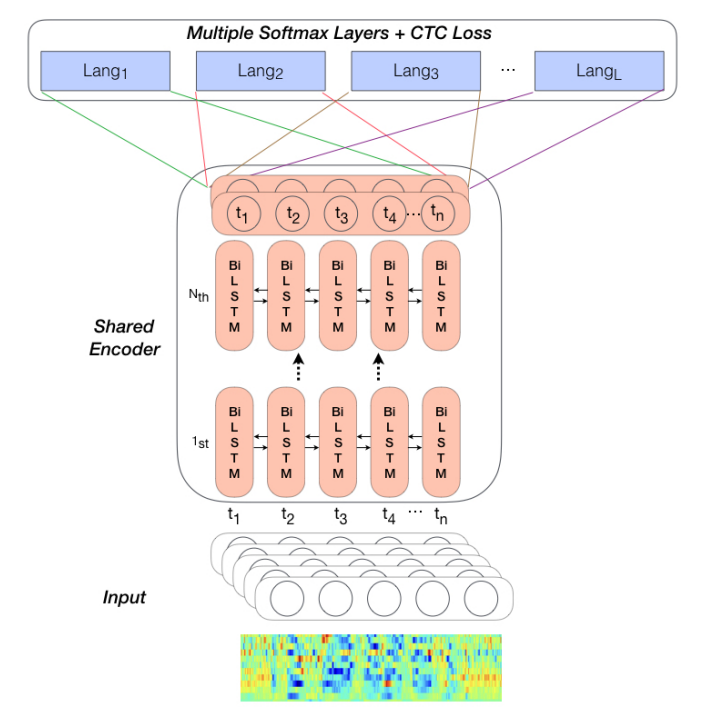
\includegraphics[width=\linewidth]{figs/model_arch.png}
    \caption{Multilingual CTC Model Architecture \textcolor{red}{WILL BE REPLACED}}
    \label{fig:model-arch}
    %\vspace{-10pt}
\end{figure}

We used the model architecture as illustrated in Fig. \ref{fig:model-arch}, parameterized by $\theta$. Let $X = x_1, x_2, \cdots, x_T$ with length $T$ as input feature, $C = c_1, c_2, \cdots, c_L$ with length $L$ as target label. $X$ is encoded into sequence of hidden states $H = h_1, h_2, \cdots, h_L$ through the shared encoder, then fed into the fully connected layer of corresponding language with softmax activation to output the prediction sequence $\hat{C} = \hat{c_1}, \hat{c_2}, \cdots, \hat{c_L}$.
%\vspace{-2pt}

\textbf{CTC Loss}. CTC computes the posterior probability as below,

\begin{equation}
  P(C|X) = \sum_{\pi \in \mathcal{Z}(C)} P(\pi|X)
\end{equation}
where $\pi$ is the repeated character sequence  of $C$ with additional blank label, and $\mathcal{Z}(C)$ is the set of all possible sequences $\pi$ given sequence $C$. For each $\pi$, we can approximate the posterior probability as below,

\begin{equation}
  P(\pi|X) \approx \prod_{i=1}^{L} P(\hat{c_i}|X)
\end{equation}

The loss function of the model is then defined as:

\begin{equation}
  \label{eq:ctc-loss}
  \mathcal{L}(\theta) = - \log P(C|X)
\end{equation}

\subsection{Meta Learning for Low-Resource ASR}

The idea of MAML is as follows. Given a set of source tasks $\mathcal{T}=\lbrace T_1, T_2, \cdots, T_K \rbrace$, MAML learns from $\mathcal{T}$ to obtain a good initialization parameter $\theta^{\star}$ achieving fast task-specific learning (fine-tuning) on target task $T_t$. In the context of ASR, we can view different languages as different tasks.

\begin{equation*}
  \theta^{\star}_t = \texttt{Learn}(T_t;\theta^{\star}) = \texttt{Learn}(T_t;\texttt{MetaLearn}(\mathcal{T}))
\end{equation*}
where $\theta^{\star}_t$ is the parameter obtained after fine-tuning on $T_t$.

\subsubsection{Learn: Language-specific learning}
Given any initial parameter $\theta^0$ (either random initialized or obtained from pretrained model) and the data of $T_t$, denoted as $D_t$. The language-specific learning process is to minimize the CTC loss function defined in Eq. \ref{eq:ctc-loss}.

\begin{equation}
  \label{eq:fine-tune}
  \resizebox{0.91\hsize}{!}{$
\begin{aligned}
  \theta^\prime = \texttt{Learn}(T_t;\theta^0) & = \arg \min_\theta \mathcal{L}_{D_t}(\theta) \\
                                 & = \arg \min_\theta \sum_{(X,C) \in D_t} -\log P(C|X)
\end{aligned}
$}
\end{equation}

The learning process is optimized through gradient descent, the same as MultiASR.

\subsubsection{MetaLearn}
The initialization parameter found by MAML should not only adapt on one language well, but for as many languages as possible. In order to achieve this goal, we define the meta learning process and the corresponding meta-objective as follows.

In each meta learning episode, we sample batch of tasks from $\mathcal{T}$, then sample two subsets from each task $k$, denoted as $D_k, D_k^\prime$. First, we use $D_k$ to simulate the language-specific learning process to obtain $\theta^\prime_k$ (\textit{inner loop}), then evaluate the effectiveness of $\theta^\prime_k$ on $D_k^\prime$. The meta-objective is defined as

\begin{equation}
  \label{eq:meta-obj}
  \mathcal{L}(\theta)=\mathbb{E}_{k \sim \mathcal{T}} \; \mathbb{E}_{D_k, D_k^\prime} \Big [\sum_{(X,C) \in D_k^\prime} - \log(C|X; \theta^\prime_k) \Big ]
\end{equation}

We then use \textit{meta gradient} obtained from Eq. \ref{eq:meta-obj} to update the model through gradient descent (\textit{outer loop}).

\begin{equation}
  \label{eq:meta-grad}
  \theta \leftarrow \theta - \eta^\prime \sum_k \nabla_\theta \mathcal{L}_{D^\prime_k}(\theta^\prime)
\end{equation}
$\eta^\prime$ is the meta learning rate.

MultiASR optimizes the model according to Eq. \ref{eq:fine-tune} on all source languages directly, without considering how learning happens on the unseen language. Although the parameter found by MultiASR is good for all source languages, it may not adapt well on the target language. Unlike MultiASR, MetaASR explicitly integrates the learning process into its framework via simulating language-specific learning first, then meta-update the model. Therefore, the parameter obtained is more suitable to adapt on the unseen language. We illustrated the concept in Fig. \ref{fig:meta-idea}, and showed in the experimental results in Section \ref{sec:results}.
